\chapter{Конструкторская часть}

В этой части представляются требования к программе,

\section{Диаграмма прецендентов}

Диаграмма прецендентов представлена на рисунке~\ref{fig:use-case-diagram}.

\begin{figure}[h!]
	\centering
	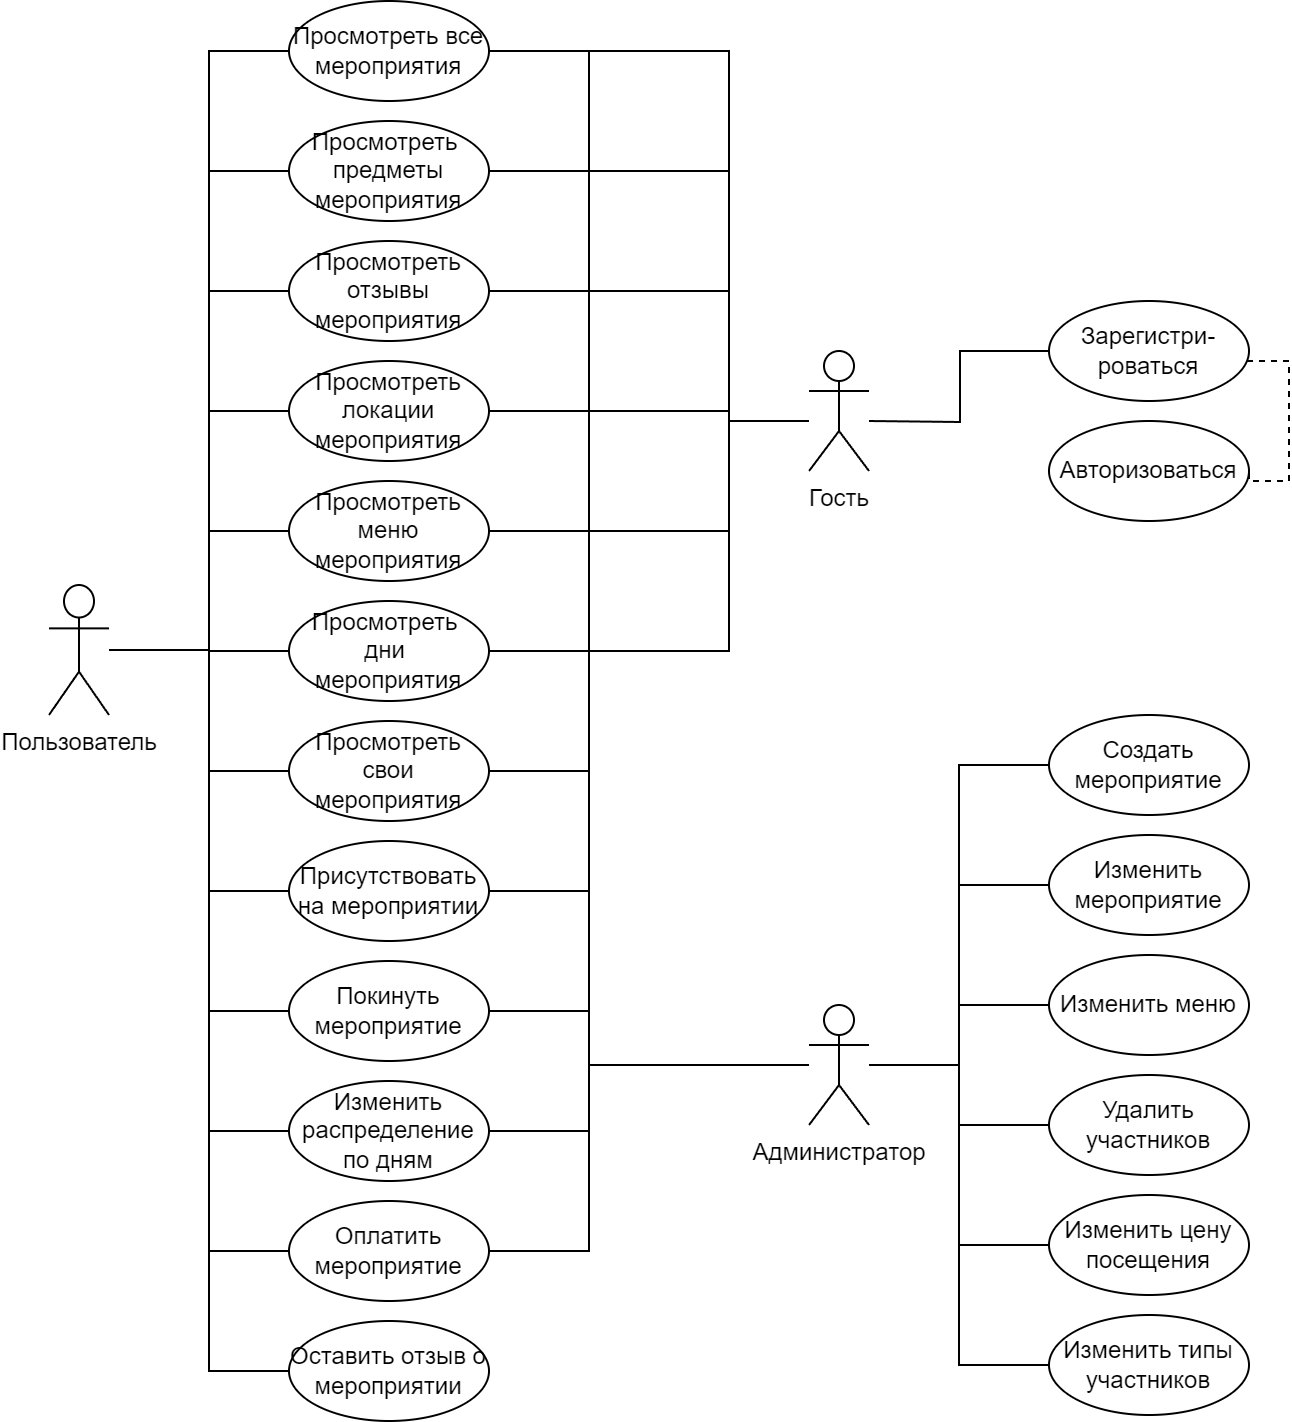
\includegraphics[width=1\textwidth]{images/use-case-diagram.png}
	\caption{Диаграмма прецендентов} 
	\label{fig:use-case-diagram} 
\end{figure}

\section{Описание сущностей базы данных}

На основе данных, представленных в таблице~\ref{tbl:data-groups}, можно определить таблицы, которые должны быть включены в базу данных:
\begin{enumerate}
	\item locations -- таблица локаций;
	\item events -- таблица мероприятий;
	\item persons -- таблица участников мероприятий;
	\item days -- таблица дней мероприятий;
	\item menu -- таблица меню дней мероприятий;
	\item items -- таблица предметов меню;
	\item feedbacks -- таблица отзывов участников;
	\item users -- таблица пользователей.
\end{enumerate}

На основе информации о выбранной СУБД и ER-диаграммы на рисунке~\ref{fig:er-diagram} можно определить структуры столбцов, их типы и ограничения для каждой таблицы, которые представлены в таблицах~\ref{tbl:locations}-\ref{tbl:users}.

\begin{table}[h!]
	\centering
	\caption{Информация о таблице локаций}
	\begin{tabularx}{\textwidth}{|p{2.6cm}|X|p{6cm}|X|}
		\hline
		\textbf{Атрибут} & \textbf{Тип данных} & \textbf{Ограничения} & \textbf{Сведение} \\
		\hline
		location\_id & UUID & NOT~NULL, \newline PRIMARY~KEY & Идентификатор локации \\
		\hline
		name & VARCHAR(255) & NOT~NULL & Название \\
		\hline
		description & TEXT & NOT~NULL & Описание \\
		\hline
		price & NUMERIC & NOT~NULL, \newline CHECK~(price~>=~0) & Цена аренды на 1 день \\
		\hline
		capacity & INT & NOT~NULL, \newline CHECK~(capacity~>=~0) & Вместимость \\
		\hline
	\end{tabularx}
	\label{tbl:locations}
\end{table}

\begin{table}[h!]
	\centering
	\caption{Информация о таблице мероприятий}
	\begin{tabularx}{\textwidth}{|p{2.6cm}|X|p{6cm}|X|}
		\hline
		\textbf{Атрибут} & \textbf{Тип данных} & \textbf{Ограничения} & \textbf{Сведение} \\
		\hline
		event\_id & UUID & NOT~NULL, \newline PRIMARY~KEY & Идентификатор мероприятия \\
		\hline
		name & VARCHAR(255) & NOT~NULL & Название \\
		\hline
		description & TEXT & NOT~NULL & Описание \\
		\hline
		date & DATE & NOT~NULL & Дата \\
		\hline
		person\_count & INT & NOT~NULL, \newline CHECK~(person\_count~>=~0) & Количество участников \\
		\hline
		days\_count & INT & NOT~NULL, \newline CHECK~(days\_count~>~0) & Количество дней \\
		\hline
		percent & NUMERIC & NOT~NULL, \newline CHECK~(percent~>=~0) & Наценка на посещение в процентах \\
		\hline
		rating & NUMERIC & NOT~NULL, \newline CHECK (rating~BETWEEN~0~AND~10) & Рейтинг \\
		\hline
	\end{tabularx}
	\label{tbl:events}
\end{table}

\begin{table}[h!]
	\centering
	\caption{Информация о таблице дней мероприятий}
	\begin{tabularx}{\textwidth}{|p{2.6cm}|X|p{6cm}|X|}
		\hline
		\textbf{Атрибут} & \textbf{Тип данных} & \textbf{Ограничения} & \textbf{Сведение} \\
		\hline
		day\_id & UUID & NOT~NULL, \newline PRIMARY~KEY & Идентификатор дня мероприятия \\
		\hline
		name & VARCHAR(255) & NOT~NULL & Название \\
		\hline
		sequence\_ number & INT & NOT~NULL, \newline CHECK (sequence\_number~>~0) & Порядковый номер \\
		\hline
		description & TEXT & NOT~NULL & Описание \\
		\hline
		price & NUMERIC & NOT~NULL, \newline CHECK~(price~>=~0) & Цена посещения \\
		\hline
	\end{tabularx}
	\label{tbl:days}
\end{table}

\begin{table}[h!]
	\centering
	\caption{Информация о таблице участников мероприятий}
	\begin{tabularx}{\textwidth}{|p{2.6cm}|X|p{6cm}|X|}
		\hline
		\textbf{Атрибут} & \textbf{Тип данных} & \textbf{Ограничения} & \textbf{Сведение} \\
		\hline
		person\_id & UUID & NOT~NULL, \newline PRIMARY~KEY & Идентификатор участника \\
		\hline
		name & VARCHAR(255) & NOT~NULL & Имя \\
		\hline
		type & ENUM & NOT~NULL & Тип \\
		\hline
		paid & BOOL & NOT~NULL & Факт оплаты \\
		\hline
	\end{tabularx}
	\label{tbl:persons}
\end{table}

\begin{table}[h!]
	\centering
	\caption{Информация о таблице меню дней мероприятий}
	\begin{tabularx}{\textwidth}{|p{2.6cm}|X|p{6cm}|X|}
		\hline
		\textbf{Атрибут} & \textbf{Тип данных} & \textbf{Ограничения} & \textbf{Сведение} \\
		\hline
		menu\_id & UUID & NOT~NULL, \newline PRIMARY~KEY & Идентификатор меню \\
		\hline
		name & VARCHAR(255) & NOT~NULL & Название \\
		\hline
		cost & NUMERIC & NOT~NULL, \newline CHECK~(cost~>=~0) & Стоимость \\
		\hline
	\end{tabularx}
	\label{tbl:menu}
\end{table}

\begin{table}[h!]
	\centering
	\caption{Информация о таблице предметов меню}
	\begin{tabularx}{\textwidth}{|p{2.6cm}|X|p{6cm}|X|}
		\hline
		\textbf{Атрибут} & \textbf{Тип данных} & \textbf{Ограничения} & \textbf{Сведение} \\
		\hline
		item\_id & UUID & NOT~NULL, \newline PRIMARY~KEY & Идентификатор предмета \\
		\hline
		name & VARCHAR(255) & NOT~NULL & Название \\
		\hline
		type & ENUM & NOT~NULL & Тип \\
		\hline
		price & NUMERIC & NOT~NULL, \newline CHECK~(price~>=~0) & Цена \\
		\hline
	\end{tabularx}
	\label{tbl:items}
\end{table}

\begin{table}[h!]
	\centering
	\caption{Информация о таблице отзывов}
	\begin{tabularx}{\textwidth}{|p{2.6cm}|X|p{6cm}|X|}
		\hline
		\textbf{Атрибут} & \textbf{Тип данных} & \textbf{Ограничения} & \textbf{Сведение} \\
		\hline
		feedback\_id & UUID & NOT~NULL, \newline PRIMARY~KEY & Идентификатор отзыва \\
		\hline
		event\_id & UUID & NOT~NULL, \newline FOREIGN~KEY & Идентификатор мероприятия \\
		\hline
		person\_id & UUID & NOT~NULL, \newline FOREIGN~KEY & Идентификатор участника \\
		\hline
		comment & TEXT & NOT~NULL & Комментарий \\
		\hline
		rating & NUMERIC & NOT~NULL, \newline CHECK (rating~BETWEEN~0~AND~10) & Рейтинг \\
		\hline
	\end{tabularx}
	\label{tbl:feedbacks}
\end{table}

\begin{table}[h!]
	\centering
	\caption{Информация о таблице пользователей}
	\begin{tabularx}{\textwidth}{|p{2.6cm}|X|p{6cm}|X|}
		\hline
		\textbf{Атрибут} & \textbf{Тип данных} & \textbf{Ограничения} & \textbf{Сведение} \\
		\hline
		user\_id & UUID & NOT~NULL, \newline PRIMARY~KEY & Идентификатор пользователя \\
		\hline
		phone & VARCHAR(255) & NOT~NULL & Телефон \\
		\hline
		gender & ENUM & NOT~NULL & Гендер \\
		\hline
		password & VARCHAR(255) & NOT~NULL & Пароль \\
		\hline
		role & ENUM & NOT~NULL & Роль \\
		\hline
	\end{tabularx}
	\label{tbl:users}
\end{table}

\newpage

Диаграмма базы данных представлена на рисунке~\ref{fig:db-diagram}.

\begin{figure}[h!]
	\centering
	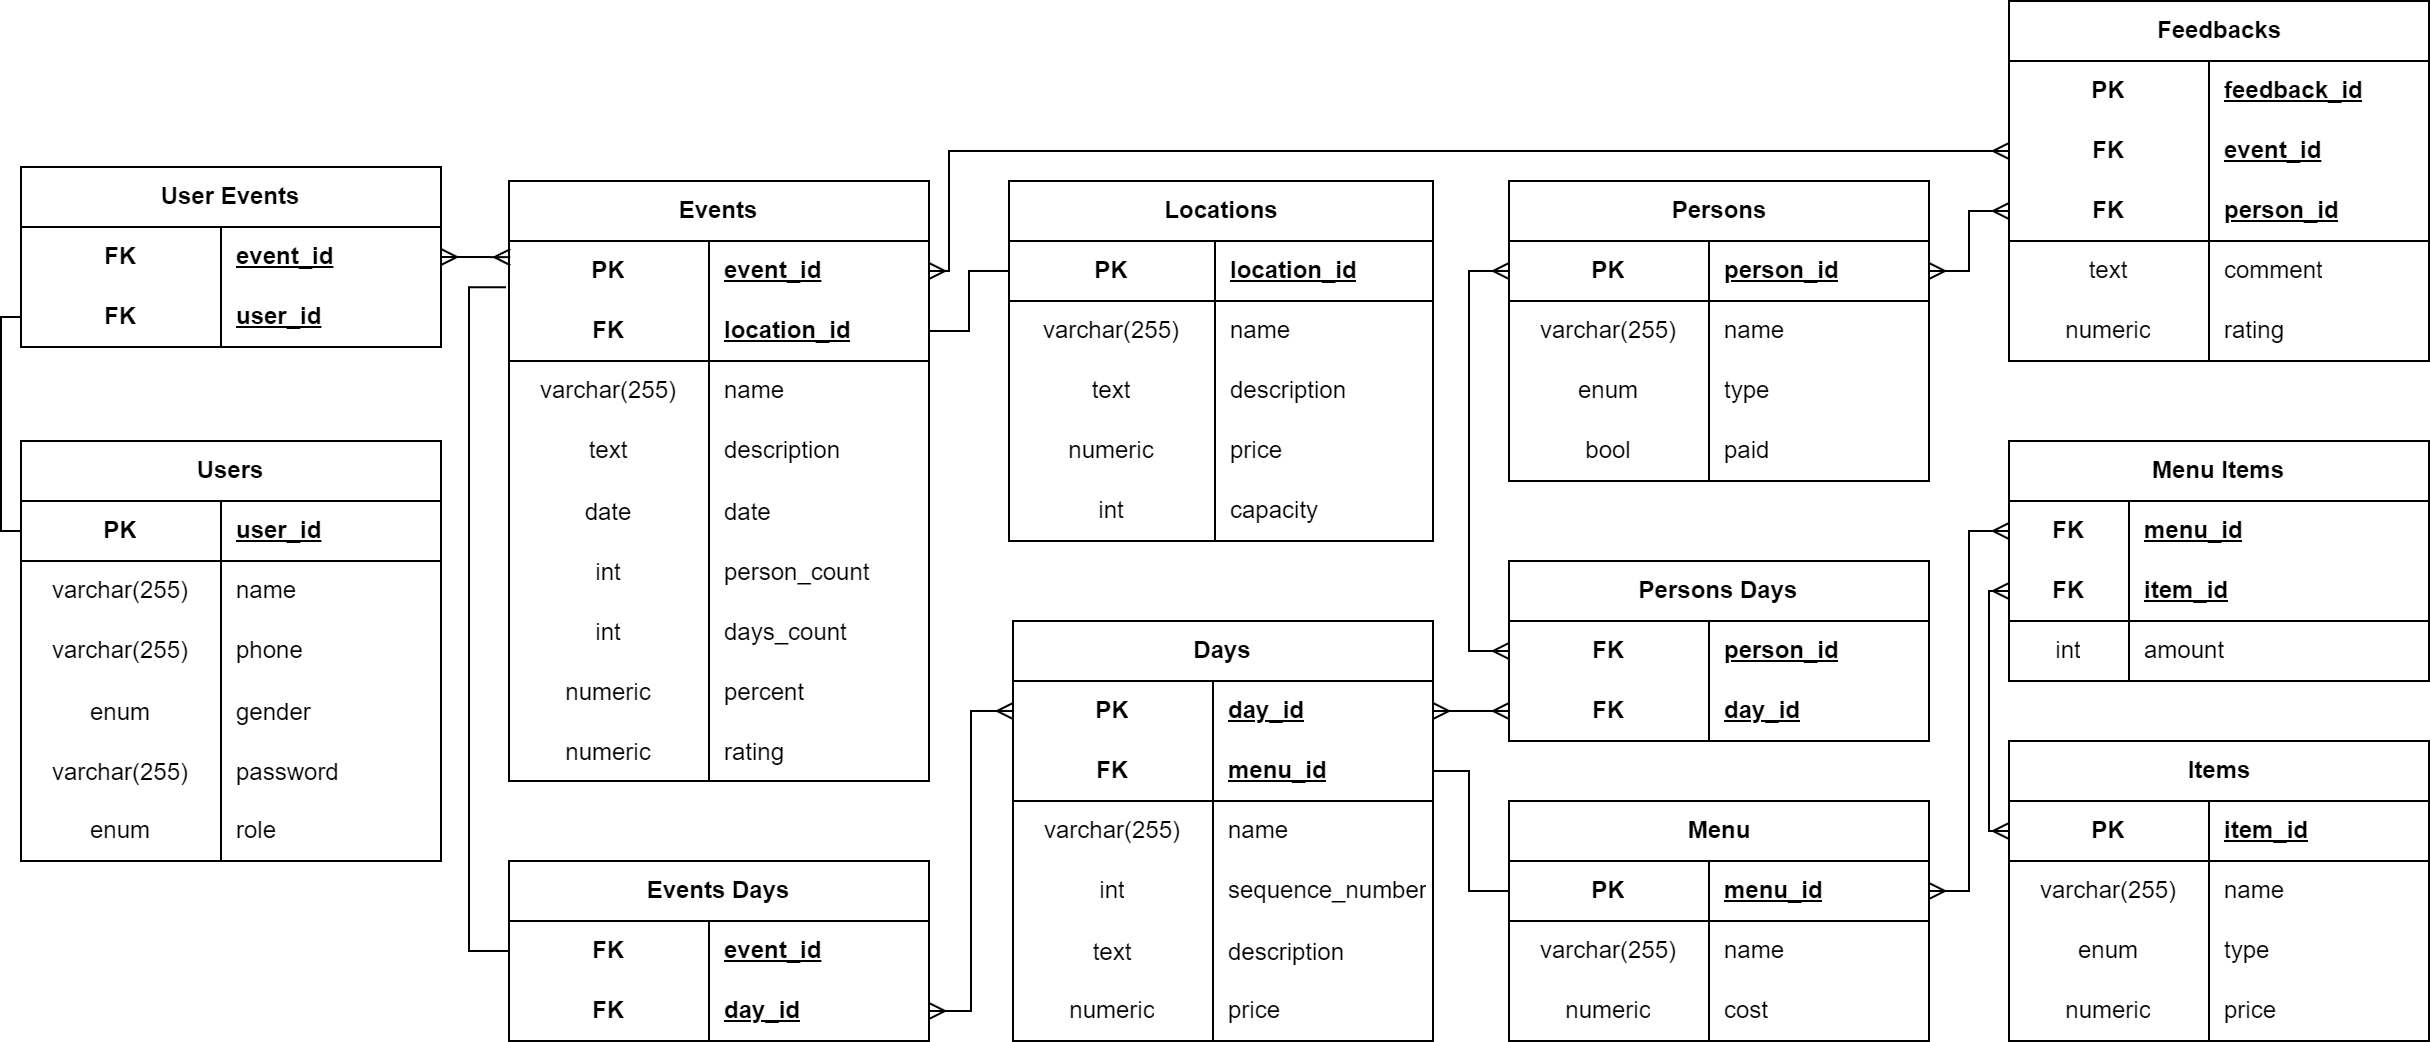
\includegraphics[width=1\textwidth]{images/db-diagram.png}
	\caption{Диаграмма базы данных} 
	\label{fig:db-diagram} 
\end{figure}

\section{Ролевая модель}

Ролевая модель в СУБД распределяет права доступа между ролями, ограничивая их действия для обеспечения безопасности:
\begin{itemize}[label=--]
	\item гость может выполнять SELECT для всех таблиц за исключением таблицы пользователей, INSERT для таблицы пользователей;
	\item авторизованный пользователь может выполнять SELECT для всех таблиц, INSERT и DELETE для таблицы мероприятий пользователей, UPDATE для таблицы пользователей;
	\item администратор имеет все права доступа.
\end{itemize}

\section{Алгоритм расчета цены посещения}

Мероприятие рассматривается как система, состоящая из участников, дней, предметов (например, еды), меню и других элементов. 

\subsection{Формализация мероприятия}

Для формализации мероприятия воспользуемся теорией множеств:
\begin{itemize}[label=--]
	\item обозначим через $P = \{p_1, p_2, \dots, p_m\}$ множество всех участников мероприятия, где $m$ -- общее количество участников. Каждый элемент $p_i$ представляет собой отдельного участника;
	\item обозначим через $D = \{d_1, d_2, \dots, d_n\}$ множество всех дней мероприятия, где $n$ -- общее количество дней. Каждый элемент $d_i$ соответствует конкретному дню;
	\item обозначим через $O = \{o_1, o_2, \dots, o_k\}$ множество всех доступных предметов (например, блюд в меню или материалов для проведения активностей), где $k$ -- общее количество предметов;
	\item обозначим через $M = \{m_1, m_2, \dots, m_n\}$ множество меню, где каждое меню $m_i$ является подмножеством множества предметов $O$, то есть \newline $m_i \subseteq O$. Каждое меню соответствует конкретному дню мероприятия;
	\item обозначим через $2^D$ булеан множества $D$, то есть множество всех возможных подмножеств дней мероприятия;
	\item определим множество $PD$ как множество упорядоченных пар $(p_i, c_j)$, где $p_i \in P$ -- участник, а $c_j \in 2^D$ -- подмножество дней, которые участник $p_i$ планирует посетить. Таким образом, $PD = \{(p_i, c_j) \mid p_i \in P, c_j \in 2^D\}$;
	\item определим множество $DM$ как множество упорядоченных пар $(d_i, m_i)$, где $d_i \in D$ -- день мероприятия, а $m_i \in M$ -- меню, соответствующее этому дню. Таким образом, $DM = \{(d_i, m_i) \mid d_i \in D, m_i \in M\}$;
	\item теперь можно определить мероприятие \( E \) как кортеж, состоящий из всех введенных множеств:  
	\begin{equation}
		E = (P, D, O, M, PD, DM)
	\end{equation}
\end{itemize}

Для расчета стоимости мероприятия и его компонентов введем следующие функции:
\begin{itemize}[label=--]
	\item обозначим через $C_O: O \rightarrow \mathbb{R}$ функцию, которая каждому предмету $o_i \in O$ ставит в соответствие его стоимость $C_O(o_i)$;
	\item определим функцию стоимости меню $C_M: M \rightarrow \mathbb{R}$ как сумму стоимостей всех предметов, входящих в меню: 
	\begin{equation}
		C_M(m) = \sum_{o_i \in m} C_O(o_i)
	\end{equation}
	\item определим функцию стоимости дня $C_D: D \rightarrow \mathbb{R}$ как стоимость меню, соответствующего этому дню:
	\begin{equation}
		C_D(d) = C_M(m), \ \text{где} \ (d, m) \in DM
	\end{equation}
	\item определим функцию стоимости мероприятия $C_E: E \rightarrow \mathbb{R}$ как сумму стоимостей всех дней мероприятия:
	\begin{equation}
		C_E(E) = \sum_{d_i \in D} C_D(d_i)
	\end{equation}
\end{itemize}

Для дальнейших расчетов введем дополнительные множества, связанные со стоимостями:
\begin{itemize}[label=--]
	\item обозначим через $C = \{c_1, c_2, \dots, c_n\}$ множество стоимостей всех дней, где $c_i = C_D(d_i)$;
	\item обозначим через $A = \{a_1, a_2, \dots, a_n\}$ множество отношений стоимостей дней к минимальной стоимости. Каждый элемент $a_i$ вычисляется по формуле:
	\begin{equation}
		a_i = \frac{c_i}{\min(C)}, \ \text{где} \ c_i \in C.
	\end{equation}
\end{itemize}

Цена посещения дня мероприятия зависит от двух факторов: стоимости дня и количества участников, которые его посещают. Введем функцию цены посещения дня $P_D: D \rightarrow \mathbb{R}$.

Стоимость дня $C_D(d)$ может быть выражена через цену посещения $P_D(d)$ и количество участников, которые планируют посетить этот день:  
\begin{equation}
	C_D(d) = P_D(d) \cdot |\{p \mid (p, d) \in PD\}|
\end{equation}
где $|\{p \mid (p, d) \in PD\}|$ -- количество участников, посещающих день $d$.

\subsection{Фундаментальная цена}

Введем понятие фундаментальной цены $P_0$, которая является константой. Фундаментальная цена -- это базовая цена, которая используется для расчета цены посещения каждого дня мероприятия. Она определяется таким образом, чтобы общая выручка от участников покрывала все затраты на проведение мероприятия. Цена посещения дня $d_i$ выражается через фундаментальную цену и отношение стоимости $a_i$:  
\begin{equation}
	P_D(d_i) = a_i \cdot P_0, \ \text{где} \ a_i \in A.
\end{equation}

Если участник планирует посетить несколько дней $\{d_i, d_j, \dots\}$, то общая цена посещения вычисляется как сумма цен каждого дня:  
\begin{equation}
	P_D(\{d_i, d_j, \cdots\}) = \sum_{d \in \{d_i, d_j, \dots\}}P_D(d) = (a_i + a_j + \dots) \cdot P_0
\end{equation}

Подставив выражение для $P_D(d_i)$ в уравнение стоимости дня, получим:
\begin{equation}
	C_D(d) = a_i \cdot P_0 \cdot |\{p \mid (p, d) \in PD\}|
\end{equation}

\section{Используемые триггеры}

\section{Архитектура приложения}

\subsection{Диаграмма потока данных}

\subsection{Диаграмма компонентов}

\subsection{Диаграмма классов}


\section{Вывод}

В конструкторской части работы были представлены требования к программе, 

\clearpage
